\graphicspath{{chapters/IGVImages/}}

\chapter{IGV (Integrative Genomics Viewer)} \label{chap: IGV}
The human genome nowadays is being explored extensively thanks to exons and
whole-genome sequencing, epigenetic surveys, expression profiling of coding and noncoding RNAs, SNPs and copy number profiling, and functional assays.\\
Those findings are essential to pave the way for the future \textbf{precision medicine}, which is an approach for disease treatment and prevention that takes into account individual variability in genes, living environment, and lifestyle for each person. The scope is to administer the right drug, at the right time and at the right dose for each individual. 

\section{Main characteristics of IGV}
Some utilization of IGV are: NGS alignment, epigenomics studies, copy number evaluations, RNA-sequencing and Identification of variants and genotypes.
Below, some of the main utilization of IGV, also represented in figur \ref{fig:IGVusages}.

\begin{figure}[H]
    \centering
    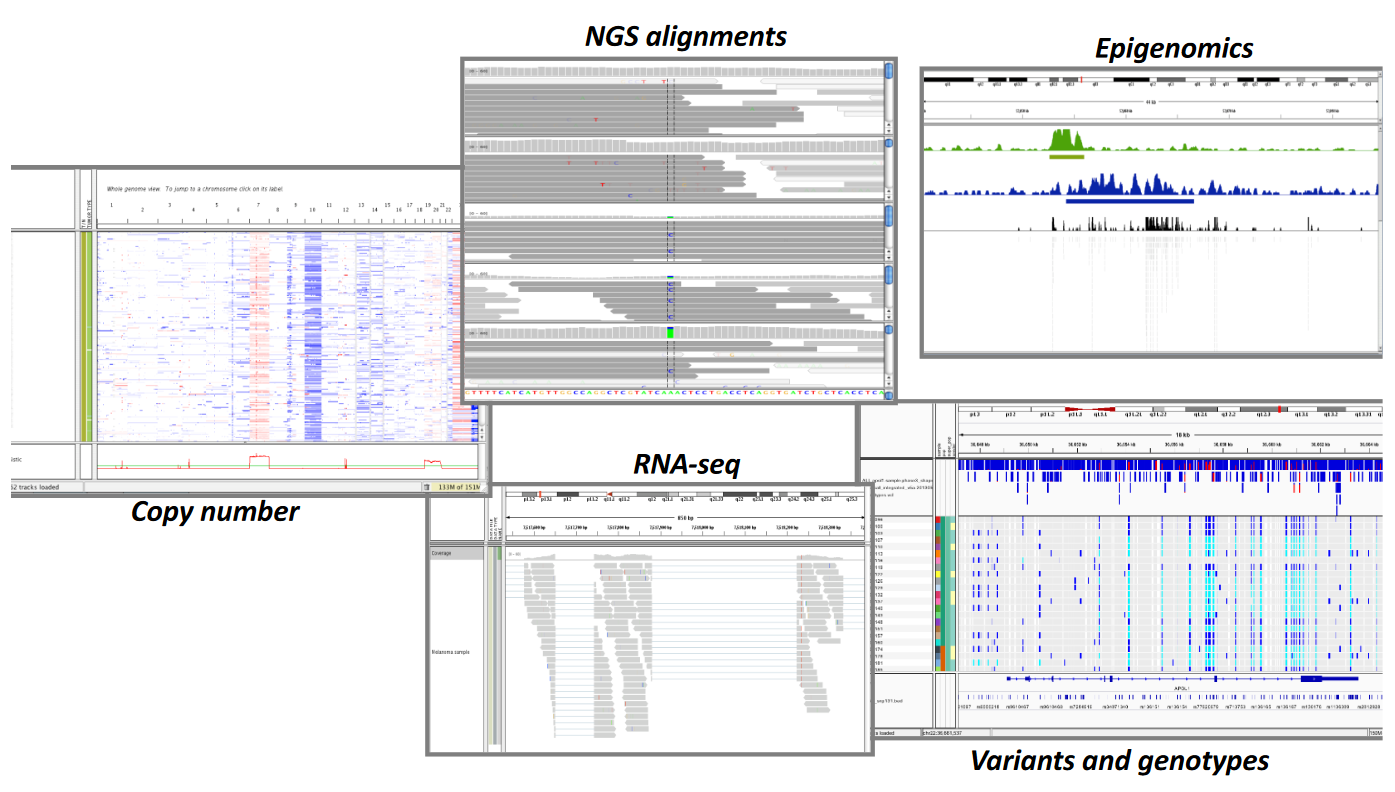
\includegraphics[width=0.8\textwidth]{usagesIGV.PNG}
    \caption{All the important usages of IGV}
    \label{fig:IGVusages}
\end{figure}

The IGV software is an \textbf{high-performance lightweight visualization tool} for interactive exploration of large, integrated genomic datasets. It supports a wide variety of data types, including next-generation sequence data, and genomic annotations. Data sets can be loaded from local or remote sources, including cloud-based resources.
\\
It allows to move, zoom in and out quickly over different genomic scales
(panel a) \ref{fig:IGV_navigation}), and also to jump in precise positions
of the sequence. It is possible to search for genomic coordinates or gene names.
For each resolution scale (“zoom level”), the aggregated data is divided into
tiles (panel b) \ref{fig:IGV_navigation}) that correspond to a region viewable on a
typical user display. Each tile is subdivided into bins, with the width of a bin
chosen to correspond to the width represented by a pixel at that resolution
scale. The corresponding data tiles for each zoom level are stored in the binary
Tiled Data Format, or TDF, which has been optimized for fast tile retrieval.\\ 
\textit{A tiled data file (\textbf{TDF}) file} (.tdf) is a binary file that
contains data that has been preprocessed for faster display in IGV. TDF files
are generated by using the \textit{igvtools} package (\textit{toTDF} command).\\

\begin{figure}[H]
\begin{tabular}{cc}
  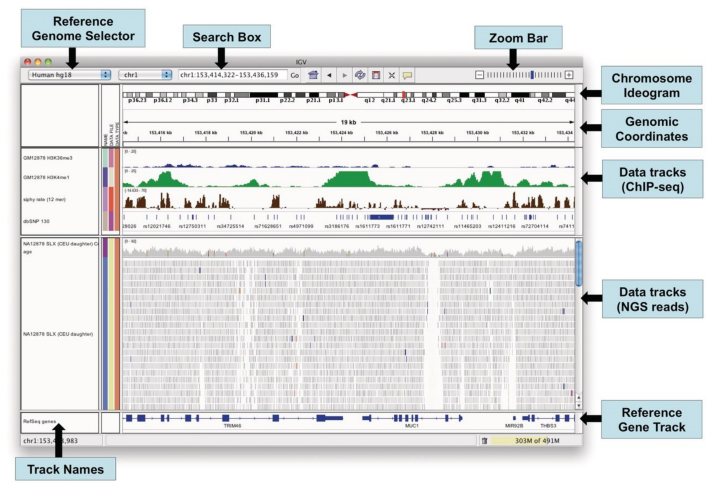
\includegraphics[width=0.5\textwidth]{IGVview.PNG} &   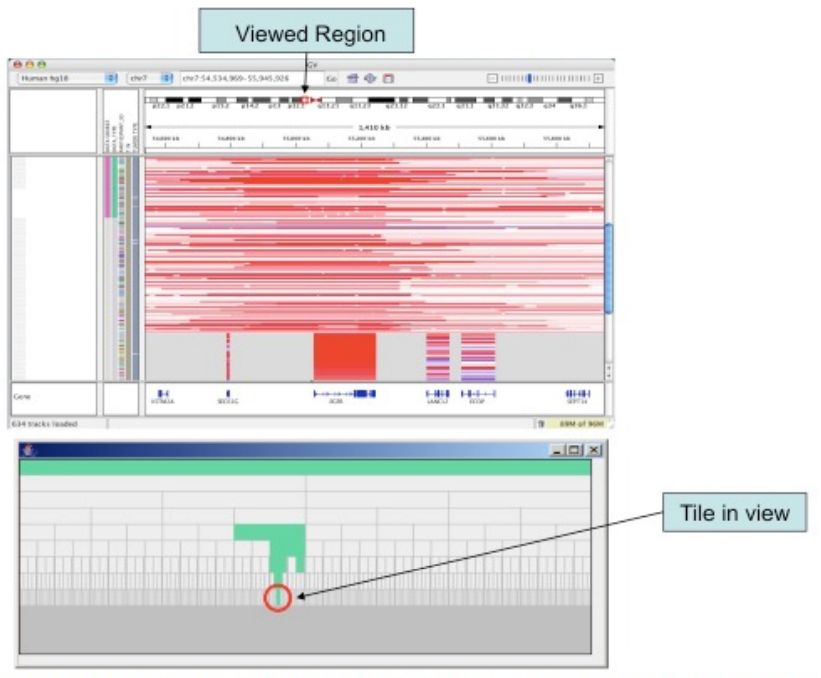
\includegraphics[width=0.5\textwidth]{TileView.PNG} \\
(a) IGV interface main features & (b) Tiles view in IGV \\[6pt]
\end{tabular}
\caption{}
\label{fig:IGV_navigation}
\end{figure}


Importantly, tile sizes for each zoom level are constant and small, and
also, a single tile at the lowest resolution (spanning the entire genome) has
the same memory footprint as a tile at the very high zoom levels (might span
only a few kilobases). \\
Tiles no longer in view are discarded as needed to free memory. Navigation
through a data set is similar to that of \textit{Google Maps}, allowing the user
to zoom and pan seamlessly across the genome at any level of detail from whole
genome to base pair.\\

\textbf{Pixel resolution errors}, occuring when data density exceeds the
constraint given by the number of pixels available for display, could be solved
through data aggregation. As the user zooms below the ~50 kb range, individual
aligned reads become visible, like in figure \ref{fig:ViewReads}. It is possible then to zoom further, and see the
bases at each position.\\
 
Annotations for specific genomes could be found consulting the UCSC Table
Browser \href{http://genome.ucsc.edu/cgi-bin/hgTables}{(UCSC table)}.\\

Other information regarding IGV are present in the
\href{https://authors.library.caltech.edu/72234/2/nbt.1754-S1.pdf}{Supplementaty
information - Integrative Genomics Viewer} pdf file.

\begin{figure}[H]
    \centering
    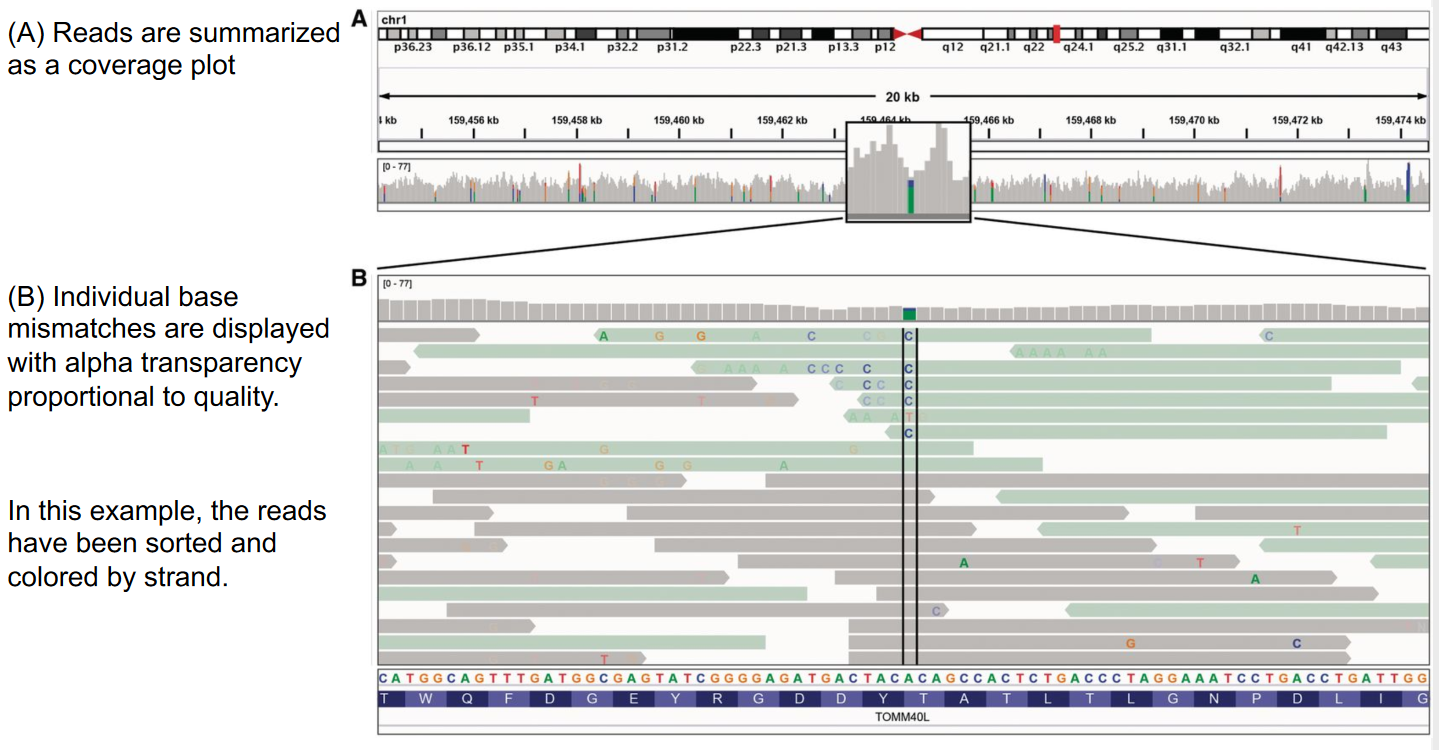
\includegraphics[width=0.7\textwidth]{IGVReadsView.PNG}
    \label{ViewReads}
    \caption{(A) Reads are summarized as a coverage plot .\\
(B) Individual base mismatches are displayed with alpha transparency proportional to quality. In this example, the reads have been sorted and colored by strand. 20 kb genomic region, 1 individual. The coverage is [0-77]; at certain positions we have more than one base supported by the reads. E.g. green and blue column, some reads support C instead of A. The colored area is proportional to the allelic fraction for each base.
}
\end{figure} 


\subsection{Igvtools}
\textit{Igvtools} comprise a set of utilities to prepare large files for efficient
display. Some commands are reported in figure \ref{fig:commands}

\begin{figure}[H]
    \centering
    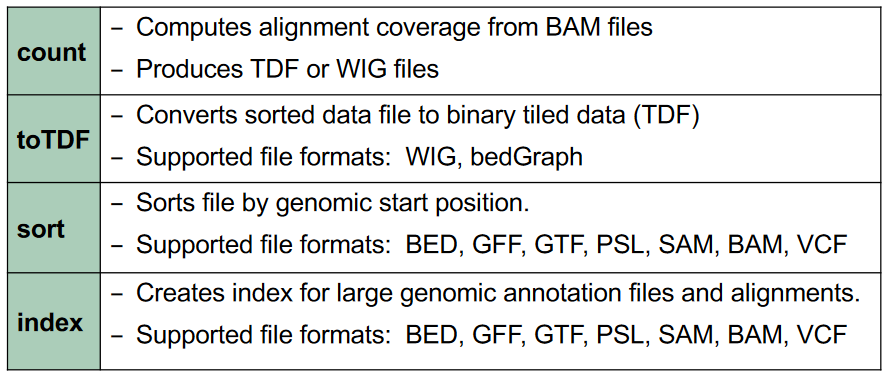
\includegraphics[width=0.6\textwidth]{igvtools.PNG}
    \caption{igvtools possible operations, the "count" function allows to generate coverage data, and it takes in input a BAM file. The obtained 
    file could be then loaded with the "Load pre-computed coverage data" command}
    \label{fig:commands}
\end{figure}

\subsection{Session Files}
Sessions allow users to share their data and views with other users simply and accurately. Session files describe the session in XML, like in figure \ref{fig:XMLfile}.

\begin{figure}[H]
    \centering
    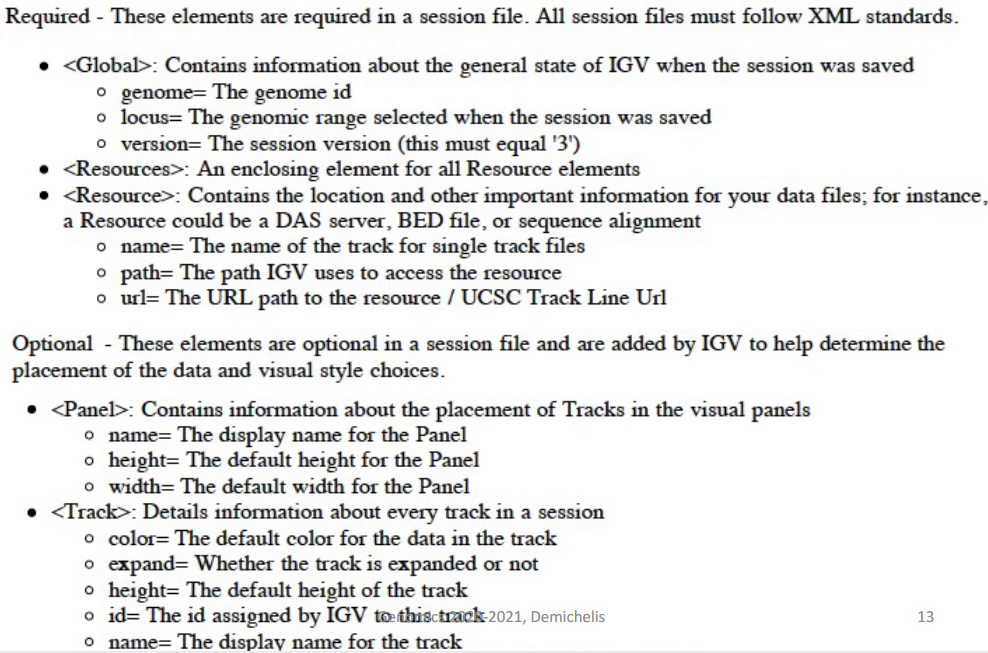
\includegraphics[width=0.8\textwidth]{structureXMLfile.PNG}
    \label{fig:XMLfile}
    \caption{Structure of the XML file}
\end{figure} 


\section{Some of the main utilizations}
\textit{(Not all the passages needed to obtain the figures are described below, as they are included in the exercise file delivered by the professor)}

\subsection{RNA-seq alignments}
\begin{figure}[H]
    \centering
    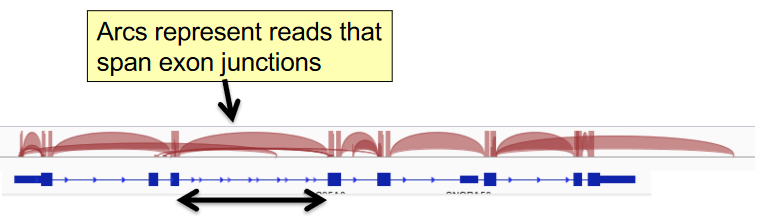
\includegraphics[width=0.8\textwidth]{RNAseqAlign.PNG}
    \caption{the height depends on the quantity of reads connecting the different exons.}
    \label{fig:RNAseq}
\end{figure}

\begin{figure}[H]
    \centering
    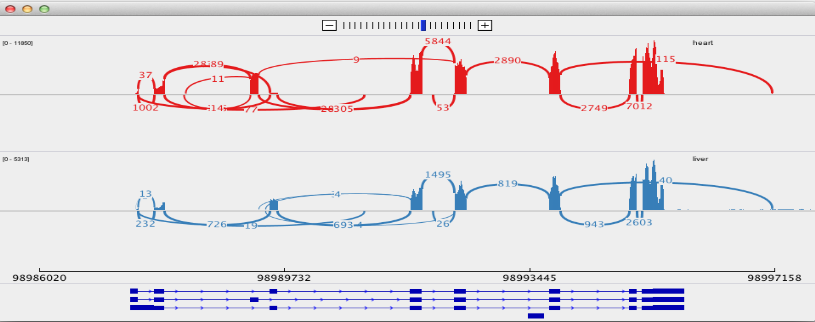
\includegraphics[width=0.8\textwidth]{sashamiplot.PNG}
    \caption{\textbf{Sashami plots}: The number of reads connecting exosomes are
    represented here on the curved lines. The peaks represent coverage within
    exons.}
    \label{fig:sashami}
\end{figure}

\subsection{Study of variants}
It is possible to study variants from different samples.
\begin{figure}[H]
    \centering
    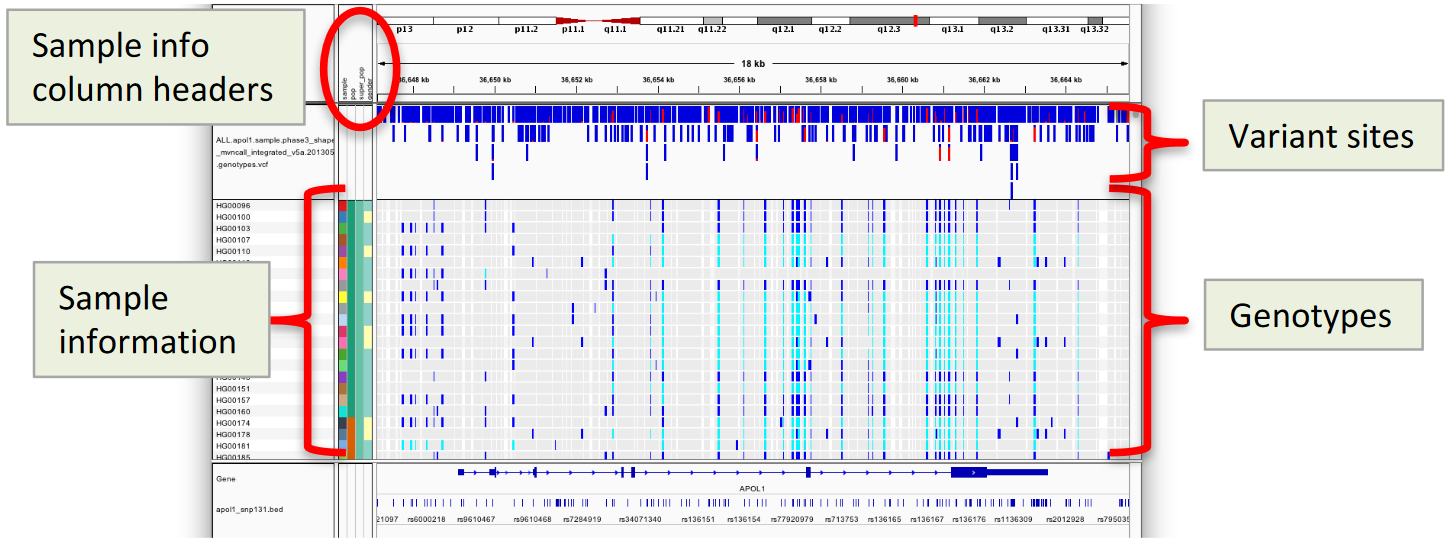
\includegraphics[width=0.9\textwidth]{variantsView.PNG}
    \label{fig:variants}
\end{figure}

It is also possible to sort the samples in different ways and to group them
considering different characteristics.


\section{Exercise}
The goal was to read pairs/end order/coverage/insert sizes at following
coordinates (reference: hg19). Then to interpret, if possible, as inversion, inverted duplication, tandem duplication, or deletion.

\begin{figure}[H]
  \centering
  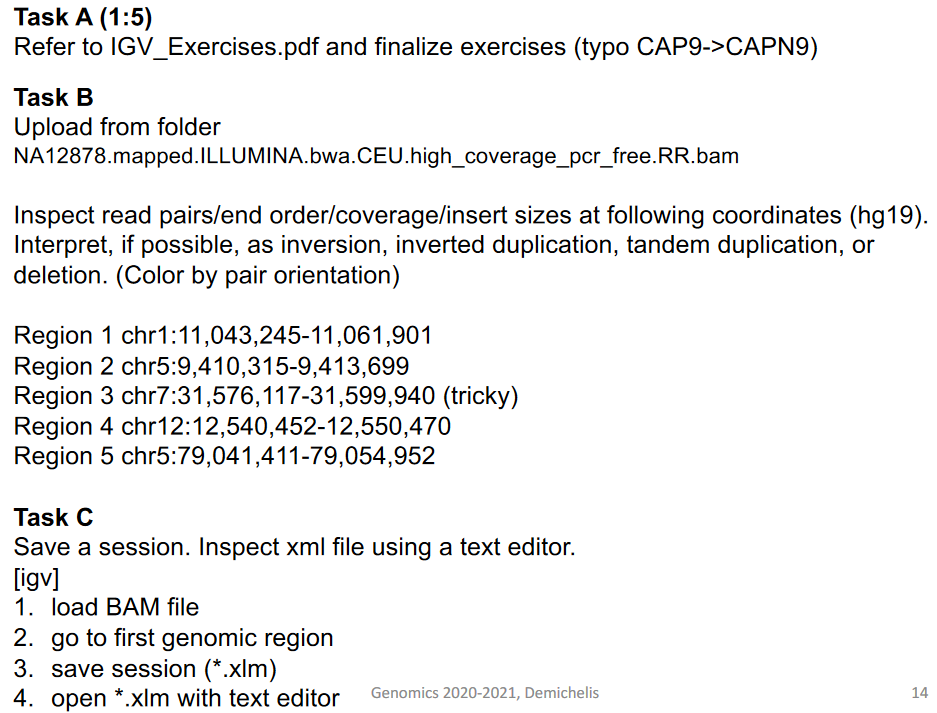
\includegraphics[width=0.6\textwidth]{TasksClass.PNG}
  \label{fig: Tasks performed IGV}
  \caption{Tasks performed}
\end{figure}

\subsection{Task B}

\begin{figure}[H]
    \centering
    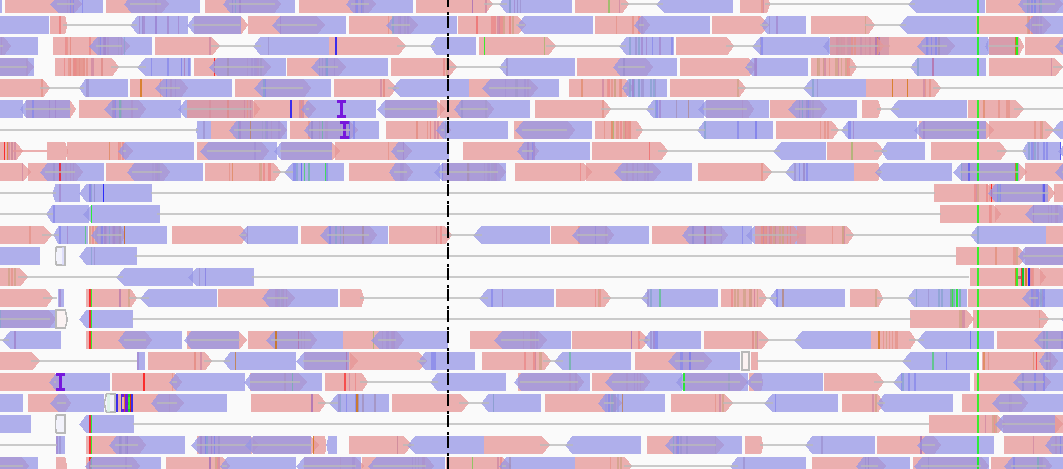
\includegraphics[width=0.8\textwidth]{pos1.PNG}
    \caption{\textit{\textbf{chr1:11,050,009-11,055,137}}: It could be a tandem
    duplication on one of the two alleles and a deletion on the other allele.
    The reason why I would suggest the presence of a deletion is due to the fact
    that the coverage remains quite constant, despite of the duplication.}
    \label{fig:task_B}
\end{figure}

\begin{figure}[H]
    \centering
    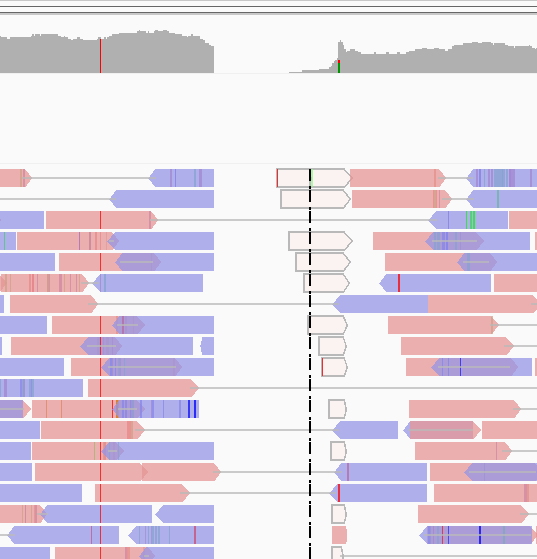
\includegraphics[width=0.8\textwidth]{pos2.PNG}
     \caption{\textbf{\textit{chr5:9,410,315-9,413,699}}: it is quite clear that
    both the alleles were deleted in that region, because of the decrease in
    coverage}
\end{figure}


\begin{figure}[t]
   \centering
   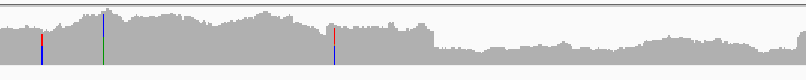
\includegraphics[width=1\textwidth]{cov3.PNG}
   \label{fig:cov3}
\end{figure}


\begin{figure}[H]
\begin{tabular}{cc}
  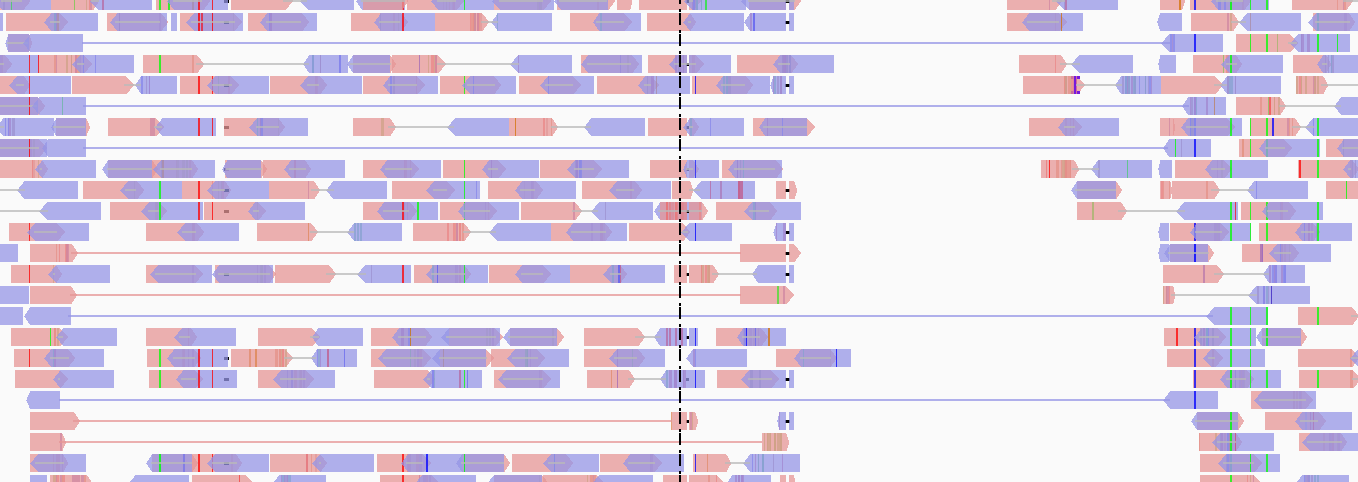
\includegraphics[width=0.5\textwidth]{pos3.PNG} &   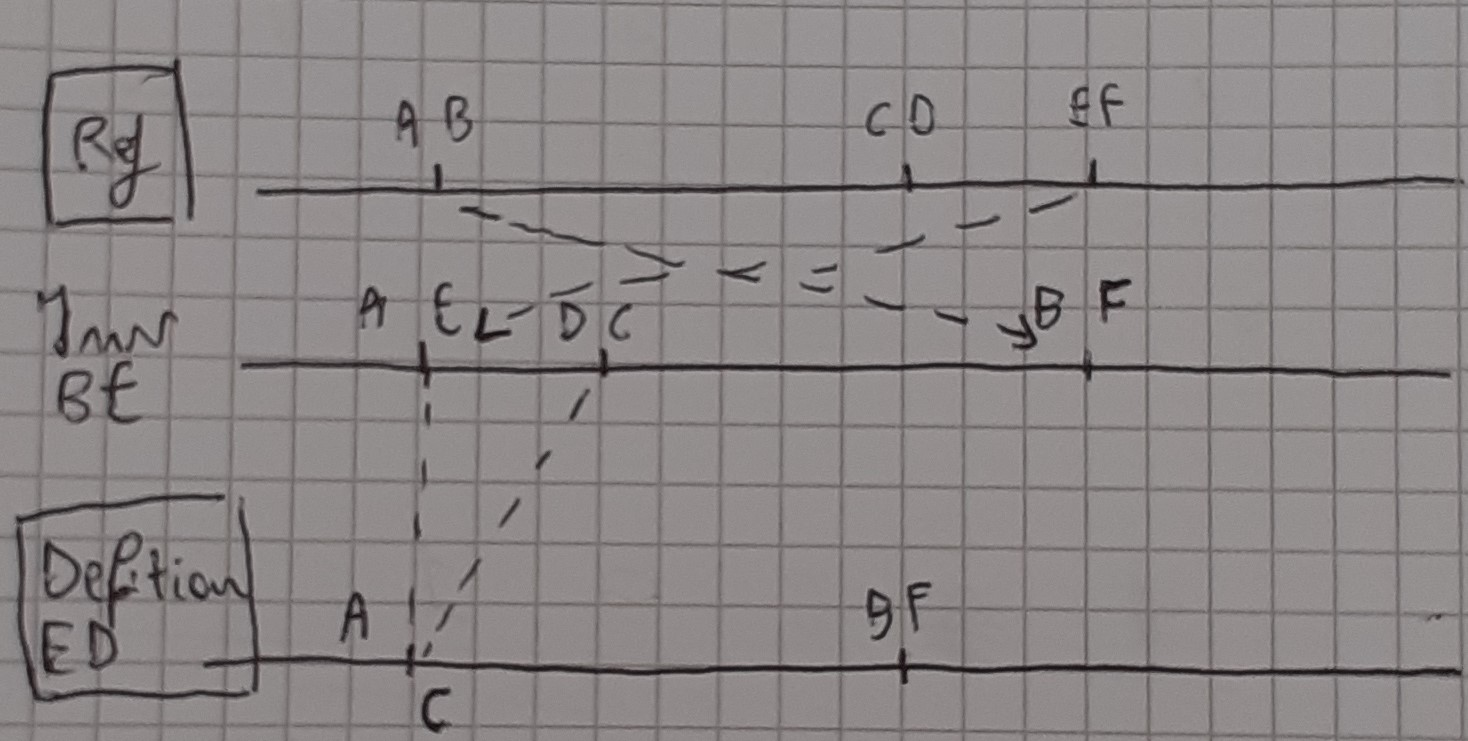
\includegraphics[width=0.5\textwidth]{pos3passages.jpg} \\
(a) IGV view & (b) written passages \\[6pt]
\end{tabular}
\caption{}
\label{fig:ex_3}
\end{figure}


%#TODO complete all the figures of the exercise #TODO it could be a good idea to
%expand this part with some information. Let me know.

